\chapter{Potláčanie multi-kamerovej interferencie ToF senzorov} 
\label{kap:interference}
\pagestyle{fancy}
\fancyhf{}
\fancyfoot[CE,CO]{\thepage}
\renewcommand{\footrulewidth}{1pt}
\lhead{Potláčanie multi-kamerovej interferencie ToF senzorov}

Jedným z nevýhod použitia ToF senzorov je ich multi-kamerová interferencia (MCI). Ide o chybu, ktorá ma fyzikálnu podstatu a má veľmi negatívny dopad na výstupné dáta. Ak pri snímaní scény nastane táto interferencia, skenovací systém sa stáva nepoužiteľným. 

Jednou z možnosti riešenia problému je použitie kamier, ktoré pracujú na rozdielnych modulačných frekvenciách emitovaného svetla. Mnoho nedávnych prác zaoberajúcich sa problémom multi-kamerovej interferencie  uvádzajú, že ToF senzory sa nesmú prevádzkovať s rovnakou modulačnou frekvenciou \cite{Kim}. Spoliehajú sa na ortogonálne funkcie, ako sú sínusoidy s rôznou frekvenčnou moduláciou. Toto riešenie je však obmedzujúce, pretože vzniká problém softvérovej kompatibility s pripojením rôznych typov kamier v jednej aplikácii \cite{Buttgen, Whyte, Seitz}.
Pomocou metódy LSENS je možné obnoviť informácie o hĺbke a amplitúde. Táto metóda je založená na analýze štatistických vlastností interferencie signálu \cite{Lianhua}. Interferenčný signál však musí mať kladné a záporné pulzovanie hĺbkovej mapy. V situáciách, keď sú kamery namierené proti sebe, môže byť kolísanie signálu extrémne vysoké. V takom prípade nebude metóda LSENS účinná. Z analýzy výstupných dát je však možné určiť podmienky potlačenia interferencie a podľa nich nevrhnúť filtračný algoritmus. Úlohou filtra je odstrániť čo najviac poškodených dát pri čo najmenšej strate relevantných dát.    


\section{Model ToF kamery}

ToF senzory sú optické snímače, ktoré poskytujú informácie o hĺbke scény. Obsahujú aktívny svetelný zdroj, ktorý generuje amplitúdovo modulovaný signál. Signál môže mať spojitý alebo impulzný charakter. Väčšina ToF kamier vyžaruje amplitúdovo modulovanú kontinuálnu vlnu (AMCW) s frekvenciou blízkou IR na osvetlenie scény. Meranie hĺbky je založené na meraní amplitúdy fázového posunu vysielaného a prijímaného modulovaného signálu (Obr. \ref{fig::tof}). Informácie o hĺbke pre každý pixel sa môžu vypočítať pomocou synchronného demodulovania prijatého modulovaného svetla v detektore. Demodulovanie sa môže uskutočniť preložením s pôvodným modulovaným signálom. Tento proces sa nazýva krížová korelácia. Všeobecne je korelačná funkcia definovaná rovnicou \ref{eq::tof::01}.

\begin{figure}[H]
	\centering
	\includegraphics[width=0.65\textwidth]{figures/tof.png}
	\caption{Princíp činnosti merania fázového posunu pri ToF kamerách \cite{Lianhua}.}
	\label{fig::tof}
\end{figure}

\begin{equation}
\label{eq::tof::01}
c(\tau) = s(t) \otimes g(t) = \lim_{T \to \infty} {\frac{1}{T}} \int_{-\frac{T}{2}}^{\frac{T}{2}}{s(t) \cdot g(t+ \tau)}dt
\end{equation}


\noindent kde $s(t)$ je prijatý optický signál a $g(t)$ je vyžiarený (pôvodný) signál. Použitím špecifických funkcií pre kamery ToF dostaneme rovnice

\begin{equation}
\label{eq::tof::02}
g(t) = \cos{\omega t}
\end{equation}

\begin{equation}
\label{eq::tof::03}
s(t) = 1+a\cdot \cos{(\omega t - \varphi)}
\end{equation}

\begin{equation}
\label{eq::tof::04}
\begin{aligned}
c(\tau) = \varphi_{sg}(\tau) =  {{\frac{a}{2}} \cdot cos(\varphi + \omega \tau)}
\end{aligned}
\end{equation}

\noindent kde $a$ je amplitúda modulácie a $\varphi$ je fázový posun.
\noindent Táto funkcia je vypočítaná pre štyri rôzne $\omega t$ argumenty, ktoré sú posunuté z 0 o $\ang{90}$.
Prijatý signál je väčšinou navrstvený na pozadí obrazu, čo vyžaduje pridanie offsetu $ b $ do korelačnej funkcie:

\begin{equation}
\label{eq::tof::05}
\begin{aligned}
C(\tau) = c(\tau) + b
\end{aligned}
\end{equation}

\begin{equation}
\label{eq::tof::06}
\begin{aligned}
C(\tau _0) = c(\tau _0) + b}=  {{\frac{a}{2}} \cdot cos(\varphi) +b \\
C(\tau _1) = c(\tau _1) + b}= - {{\frac{a}{2}} \cdot sin(\varphi) +b \\
C(\tau _2) = c(\tau _2) + b}=- {{\frac{a}{2}} \cdot cos(\varphi) +b \\
C(\tau _3) = c(\tau _3) + b}= {{\frac{a}{2}} \cdot sin(\varphi) +b 
\end{aligned}
\end{equation}

\noindent S týmito štyrmi vybranými bodmi je možné vypočítať korelačnú funkciu a určiť fázu $\varphi$ a amplitúdu $a$ prijatého signálu $s(t)$:

\begin{equation}
\label{eq::tof::07}
\begin{aligned}
\varphi = atan \Bigg[ {\frac{C(\tau _3) - C(\tau _1)}{C(\tau _0) - C(\tau _2)}} \Bigg]
\end{aligned}
\end{equation}

\begin{equation}
\label{eq::tof::08}
\begin{aligned}
a =  \frac{\sqrt{{[C(\tau _3) - C(\tau _1)}]^2 + [{C(\tau _0) - C(\tau _2)}]^2}}{2}  
\end{aligned}
\end{equation}


\noindent Hĺbka $d$ sa vypočíta podľa nasledujúcej rovnice:


\begin{equation}
\label{eq::tof::09}
\begin{aligned}
d = \frac{ c \cdot \varphi }{ 2 \cdot 2 \pi f}
\end{aligned}
\end{equation}

\noindent kde $c$ je rýchlosť svetla a $f$ je frekvencia modulácie IR \cite {Lange}.


\section{Model multi-kamerovej interferencie}

V multi-kamerovom režime každý ToF senzor používa rovnakú modulačnú frekvenciu a IR vlnovú dĺžku, takže prijaté signály interagujú navzájom. V experimentálnej topológii senzorov používame tri ToF senzory S1 \, - \, S3, ktoré sú statické a umiestnené v skenovacej kabíne. Tento systém je znázornený na obrázku \ ref {fig: imodel}, ktorý popisuje vzájomné vzťahy medzi jednotlivými kamerami a objektom.

\begin{figure}[H]
	\centering
	\includegraphics[width=0.74\textwidth]{figures/interference_model.png}
	\caption{Model multi-kamerového systému s interferenciou IR signálu.}
	\label{fig:imodel}
\end{figure}  

Každá kamera generuje signál $g(t)$ a prijíma odrazený signál $s(t)$, ktorý predstavuje spojenie generovaných čiastkových signálov zo všetkých kamier $S$. Tieto signály možno opísať takto:

\begin{equation}
\label{eq::tof::10}
\begin{aligned}
s_1 (t) }= {s_{11}(t)+s_{12}(t)+s_{13}(t) \\
s_2 (t) }= {s_{21}(t)+s_{22}(t)+s_{23}(t) \\
s_3 (t) }= {s_{31}(t)+s_{32}(t)+s_{33}(t) 
\end{aligned}
\end{equation}

\noindent  Každý čiastkový signál možno zapísať ako:

\begin{equation}
\label{eq::tof::11}
\begin{aligned}
s_{xy}(t) = b_{xy}+a_{xy} \cdot cos(\omega t - \varphi _{xy})
\end{aligned}
\end{equation}

Index $x$ predstavuje cieľovú kameru a index $y$ kameru pôvodného signálu. Nasledujúce rovnice slúžia ako príklad výpočtu modelu pre jeden signál $s_1$. Pre ostatné kamery sa matematický model odvodzuje rovnakým spôsobom:

\begin{equation}
\label{eq::tof::12}
\begin{aligned}
&{s_{1}(t) }= {b_{11}+a_{11} \cdot cos(\omega t - \varphi _{11}) + {b_{12} +a_{12} \cdot cos(\omega t - \varphi _{12})}} \\ 
&+ {{b_{13}+a_{13} \cdot cos(\omega t - \varphi _{13})} = \Tilde{b}_1 + \Tilde{a}_1 \cdot cos(\omega t - \Tilde{\varphi_1})}  
\end{aligned}
\end{equation}

\noindent  Po 4-fázovej korelácii rušivých signálov sa rovnice \ref{eq::tof::07} a \ref{eq::tof::08} transformujú do nasledujúcej podoby:

\begin{equation}
\label{eq::tof::13}
\begin{aligned}
&{ \Tilde{\varphi}_1}= atan \Bigg[ {\frac{a_{11}  sin( \tau _{11}) + a_{12}  sin( \tau _{12}) + a_{13}  sin( \tau _{13})}{a_{11}  cos( \tau _{11}) + a_{12}  cos( \tau _{12}) + a_{13}  sin( \tau _{13}) }} \Bigg]
\end{aligned}
\end{equation}

\begin{equation}
\label{eq::tof::14}
\begin{aligned}
&\Tilde{ a_1 }= {\sqrt{\frac{a_{11}^2+a_{12}^2+a_{13}^2 + 2\bar{a}}{2} }}
\end{aligned}
\end{equation}

\noindent kde

\begin{equation}
\label{eq::tof::15}
\begin{aligned}
&{\bar{a}} = {a_{11}a_{12}[sin({\varphi_{11}+\varphi_{12}}) + cos({\varphi_{11}+\varphi_{12}})]} + \\  
&{a_{11}a_{13}[sin({\varphi_{11}+\varphi_{13}}) + cos ({\varphi_{11}+\varphi_{13}})]} + \\
&{a_{12}a_{13}[sin({\varphi_{12}+\varphi_{13}}) + cos ({\varphi_{12}+\varphi_{13}})]}
\end{aligned}
\end{equation}

Toto zmiešanie signálov z rôznych kamier spôsobuje značné chyby merania a preto mapa výstupnej hĺbky obsahuje artefakty \cite{Lianhua}.

\section{Analýza multi-kamerovej interferencie}

Rovnice \ref{eq::tof::13} a \ref{eq::tof::14} sú platné, ak každý prijatý signál $s_{x}(t)$ je kombináciou čiastkových signálov všetkých kamier S1\, - \,S3, kde $x$ sa pohybuje od 1 do 3.
Interakcia signálov úzko súvisí aj so snímanou scénou. Ak si predstavíme priestorové rozloženie kamier, ktoré je znázornené na obr. \ref{fig:imodel}, môžeme popísať určité situácie nastávajúce pri skenovaní. Ak sa v scéne nenachádza objekt, je veľmi veľká pravdepodobnosť že k interferencii dôjde medzi kamerami $s_{32}$ a $s_{23}$. Taktiež ak je veľkosť objektu malá a vyžarovanému IR svetlu nebude v ceste stáť žiadna prekážka. Naopak veľký objekt môže zabrániť interferencii medzi kamerami $s_{32}$ a $s_{23}$. Veľmi rizikové su aj predmety a povrchy, ktoré reflektujú IR svetlo. Pri skenovaní dynamických objektov sa môže vplyv rušenia meniť, takže filtračný algoritmus musí reagovať na zmeny v čo najkratšom čase.

Ako už bolo spomenuté, výstupom ToF kamier je IR a hĺbkový obraz.  Hĺbkový obraz obsahuje 3D informácie v 2D rovine obrazu. Hodnota jednotlivých pixelov (32-bit float) predstavuje absolútnu vzdialenosť. Na základe týchto informácií je možné znovu premietať naskenovanú scénu, kde musia byť známe interné a externé parametre IR kamery (pozri kapitolu \ref{kap:kalibracia}).

\begin{figure}[h]
	\centering
	\begin{subfigure}[b]{0.2\textwidth}
		\centering
		\includegraphics[width=\textwidth]{figures/depth_ir-a.png}
		\caption{}
		\label{fig:depthir:a}
	\end{subfigure}
	\hfill
	\begin{subfigure}[b]{0.2\textwidth}
		\centering
		\includegraphics[width=\textwidth]{figures/depth_ir-b.png}
		\caption{}
		\label{fig:depthir:b}
	\end{subfigure}
	\hfill
	\begin{subfigure}[b]{0.2\textwidth}
		\centering
		\includegraphics[width=\textwidth]{figures/depth_ir-c.png}
		\caption{}
		\label{fig:depthir:c}
	\end{subfigure}
	\hfill
	\begin{subfigure}[b]{0.2\textwidth}
		\centering
		\includegraphics[width=\textwidth]{figures/depth_ir-d.png}
		\caption{}
		\label{fig:depthir:d}
	\end{subfigure}
	\caption{Obrazy zo senzora Microsoft Kinect v2: (\textbf{a}) IR obraz bez interferencie. (\textbf{b}) IR obraz s interferenciou. (\textbf{c}) Hĺbková mapa IR obrazu (a). (\textbf{d}) Hĺbková mapa IR obrazu (b). Miesto interferencie je zvýraznené červenou farbou.}
	\label{fig:depthir}
\end{figure}

Interferencia sa prejavuje na IR obraze, čo ma priamy dopad na výsledný hĺbkový obraz (pozri obr. \ref{fig:depthir}). V hĺbkovom obraze sa v poškodenom mieste objavia pixely, ktoré naberajú extrémne odlišné hodnoty od tých skutočných. Tie sú buď negatívne alebo pozitívne, pričom sa zvyknú pulzovaním striedať. 

\begin{figure}[h]
	\centering
	\begin{subfigure}[b]{0.24\textwidth}
		\centering
		\includegraphics[width=0.7\textwidth]{figures/3dmodels-c.png}
		\caption{}
		\label{fig:3dm:b}
	\end{subfigure}
	\hfill
	\begin{subfigure}[b]{0.24\textwidth}
		\centering
		\includegraphics[width=0.7\textwidth]{figures/3dmodels-a.png}
		\caption{}
		\label{fig:3dm:a}
	\end{subfigure}
	\hfill
	\begin{subfigure}[b]{0.24\textwidth}
		\centering
		\includegraphics[width=0.7\textwidth]{figures/3dmodels-d.png}
		\caption{}
		\label{fig:3dm:d}
	\end{subfigure}
	\hfill
	\begin{subfigure}[b]{0.24\textwidth}
		\centering
		\includegraphics[width=0.7\textwidth]{figures/3dmodels-b.png}
		\caption{}
		\label{fig:3dm:c}
	\end{subfigure}
	\caption{Rekonštruovaný 3D model statického objektu: (\textbf{a}) 3D trojuholníková sieť objektu bez interferencie. (\textbf{b}) 3D trojuholníková sieť objektu s interferenciou. (\textbf{c}) Mračno bodov objektu bez interferencie. (\textbf{d}) Mračno bodov objektu s interferenciou.}
	\label{fig:3dmodel}
\end{figure}

Pri pozitívnej interferencii môže ísť hĺbka do maximálnych možných hodnôt (32-bit float), pri negatívnej môže ísť do 0. Tieto miesta sú zároveň obkolesené deformovanými pixelmi, ktoré nenaberajú extrémne hodnoty, ale stále výrazne zhoršujú kvalitu výstupného modelu. Grafické znázornenie v 3D priestore je možné vidieť na obrázkoch \ref{fig:3dm:b} a \ref{fig:3dm:d}. Práve tieto miesta sú veľmi kritické, pretože ich identifikácia je problematická. 

\section{Filtračné metódy}
\label{sec:filtmethods}

Existuje niekoľko prehľadových článkov, ktoré sa zaoberajú technikami filtrácie a obnovy používanými pri 3D zobrazovaní a skenovaní. Zo všetkých z nich sa práca \cite{Han} javí ako veľmi užitočná, pretože obsahuje prehľad približne 40 metód a rozdeľuje ich do niekoľkých tried. Mnohé z týchto metód sú použiteľné na 3D mračná bodov, avšak žiadny známy nie je priamo určený pre potláčanie interferencie. Na tento účel bol navrhnutý IMBM filter, ktorý sa môže zaradiť medzi štatistické filtre. Pre porovnanie sú v tejto práci opísané ďalšie filtračné metódy založené na štatistike (SOR, ROR) alebo na princípoch umelej inteligencie (PointCleanNet).   

\subsection{SOR filter}

Filtračná metóda SOR (Statistical Outlier Removal) je založená na štatistickej analýze okolia každého bodu. Odľahlá hodnota sa dá klasifikovať ako stratený alebo izolovaný bod, poprípade ako súbor bodov v mračne. V SOR metóde sa určuje počet bodov, ktoré sa budú považovať za susedov (definovaný počet $k$ najbližších susedov \cite{Pirotti}) a potom sa vypočíta priemerná vzdialenosť každého bodu od jeho susedov. Body, ktorých stredné vzdialenosti nespĺňajú kritériá a sú mimo intervalu sa považujú za odľahlé. Interval je definovaný strednou hodnotou stredných vzdialeností a štandardnou odchýlkou \cite{Corso}. SOR je široko používaná a efektívna metóda, aj keď vo veľkých množinách 3D dát je časovo neefektívna  \cite{Balta}.

\subsection{ROR filter}
Metóda ROR (Radius Outlier Removal) predstavuje pomerne jednoduchý štatistický filter. Do filtra sa zadávajú parametre sférického polomeru $rad$ a minimálneho počtu susedov $pts$. Filter odstráni body, ktoré majú v oblasti polomeru $rad$ menej susedných bodov ako bolo nastavené parametrom $pts$.


\subsection{PointCleanNet}
PointCleanNet je dvojfázový algoritmus hĺbkového učenia, ktorý odstraňuje odľahlé hodnoty a znižuje šum v neusporiadaných mračnách bodov. Architektúra je založená na PCPNet (prístup založený na hlbokom učení na odhad lokálnych 3D vlastností v mračnách bodov \cite{Guerrero}) s niekoľkými úpravami. V prvom kroku sa odstraňujú odľahlé body, v druhom sa odhadujú korekčné vektory pre zostávajúce body. Trénovanie tejto siete je časovo náročné, taktiež je vyžadované použitie CUDA.

\subsection{Importance Map Based Median filter}

Nami navrhnutý filtračný algoritmus je založený na identifikácií, extrakcii a interpolácií interferenčnej oblasti zo sekvencie hĺbkových máp získaných z ToF senzorov. Cieľom nie je poškodené miesta úplne odstrániť, ale čo najviac minimalizovať vplyv interferencie bez veľkej straty užitočných dát. Primárne využitie filtra je pre aplikáciu skenovania ľudských hláv, ale nie je obmedzené iba na túto činnosť. Základnou požiadavkou je získať dostatočný počet hĺbkových máp do obrazového zásobníka, pričom snímaná scéna nebola výrazne zmenená. Táto podmienka je splnená, ak je snímaný objekt statický alebo v pokoji (pacient nie je v strese). V prípade dynamickej scény je žiadúca minimalizácia veľkosti zásobníka, inač by mohlo dôjsť k vytvoreniu pohybových artefaktov v hĺbkovej mape.

\begin{figure}[h]
	\centering
	\includegraphics[width=0.75\textwidth]{figures/algorithm.png}
	\caption{Blokový diagram navrhnutého IMBM filtra.}
	\label{fig:algorithm}
\end{figure}

V prvom kroku je potrebné naplniť obrazový zásobník, ktorého veľkosť je špecifikovaná podľa danej snímanej scény a intenzity interferencie. Plnenie funguje na princípe FIFO. Najprv sa zásobník naplní hĺbkovými mapami a po naplnení zásobníka každý nový snímok vylúči ten najstarší, čím je zabezpečená stála veľkosť zásobníka. 
Všetky vstupujúce hĺbkové mapy sú prahované podľa prahových hodnôt určených topológiou a vlastnosťami systému.  

Ak \textit{d(x;y)} predstavuje jednotlivý pixel hĺbkovej mapy, tak je prahovanie vykonávané pomocou rovnice \ref{eq::imbm::threshold}.

\begin{equation}
\label{eq::imbm::threshold}
\begin{aligned}
d'(x;y)=
\begin{cases}
d(x;y), & \text{if}\ d(x;y) \in < T_{LOW}; T_{HIGH}> \\
0, & \text{v inom prípade}
\end{cases}
\end{aligned}
\end{equation}

kde \textit{d(x; y)} je 32-bitové float číslo a $T_{LOW}$, $T_ {HIGH}$ sú dolné a horné prahové hodnoty. V našom prípade sú nastavené na 80 a 1300 (tieto čísla predstavujú skutočnú vzdialenosť v mm). Skenovacia kabína je znázornená na obrázku \ref {fig:cabin} a rozmer spodnej časti je $ 1520 \times 1520$ \, mm.

\begin{figure}[h]
	\centering
	\begin{subfigure}[b]{0.49\textwidth}
		\centering
		\includegraphics[height=5.5cm]{figures/threshold_a.png}
		\caption{}
		\label{fig:threshold:a}
	\end{subfigure}
	\hskip 0pt
	\begin{subfigure}[b]{0.49\textwidth}
		\centering
		\includegraphics[height=5.5cm]{figures/threshold_b.png}
		\caption{}
		\label{fig:threshold:b}
	\end{subfigure}
	\caption{Vplyv prahovania na interferovanú hĺbkovú mapu(\textbf{a}) Hĺbková mapa s interferovanými regiónmi. Pixely nadobúdajú extrémne hodnoty. (\textbf{b}) Hĺbková mapa bez extrémnej interferencie.}
	\label{fig:threshold}
\end{figure}

Po prahovaní hĺbky sa pozadie odstráni a obrázky obsahujú iba predmet záujmu (Obr. \, \ref{fig:threshold}). Tento jednoduchý krok je dôležitý a účinný, pretože odstraňuje oblasti so spomínanou extrémnou interferenciou a pozadia.

V ďalšom kroku sa z obrazového zásobníka vyberie ako referenčný obraz filtrovaná hĺbková mapa s minimálnym počtom nenulových hodnôt. Je to preto, že tento obrázok s najväčšou pravdepodobnosťou obsahuje minimálny počet rušivých pixelov. Z tejto referencie je vytvorená binárna mapa a každá hĺbková mapa je s ňou maskovaná. V tomto kroku sú pixely vstupných máp rozdelené do troch oblastí: pozadie (vrátane extrémnych interferenčných oblastí), pixely interferenčnej oblasti (tiež vrátane niektorých pixelov objektu) a oblasť objektov (vrátane interferenčných pixelov).


\begin{figure}[h]
	\centering
	\begin{subfigure}[b]{0.32\textwidth}
		\centering
		\includegraphics[height=5.2cm]{figures/interf_roi_a.png}
		\caption{}
		\label{fig:interf:a}
	\end{subfigure}
	\hskip 0pt
	\begin{subfigure}[b]{0.32\textwidth}
		\centering
		\includegraphics[height=5.2cm]{figures/interf_roi_b.png}
		\caption{}
		\label{fig:interf:b}
	\end{subfigure}
	\hskip 0pt
	\begin{subfigure}[b]{0.32\textwidth}
		\centering
		\includegraphics[height=5.2cm]{figures/interf_roi_c.png}
		\caption{}
		\label{fig:interf:c}
	\end{subfigure}
	\caption{Identifikácia interferovaných regiónov v hĺbkových mapách. (\textbf{a}) Referenčná mapa s maximálnym počtom 0 pixelov.(\textbf{b}) Vstupná mapa s interferenciou. (\textbf{c}) Mapa zobrazujúca možné interfereované regióny obrazu \textbf{b}.}
	\label{fig:interf}
\end{figure}


Výsledná rozdielová maska je ešte dilatovaná prvkom o štvorcovej štruktúre $ 1 \times1 $, čím sú odstraňované oblasti s nízkou intenzitou interferencie. Týmto spôsobom sa zníži celkový súčet interferenčných pixelov, ale zároveň znižujeme aj súčet správnych obrazových pixelov skenovaného objektu. 

Tieto morfologicky spracované snímky sa používajú na výpočet mediánu hĺbkovej mapy a na vytvorenie mapy dôležitosti pixelov.\newline


\textbf{Pixel mediánu hĺbkovej mapy} je vypočítavaný ako medián všetkých konkrétnych nenulových pixelov (rovnaká pozícia riadku a stĺpca v obraze) hĺbkových máp v zásobníku. \newline

\textbf{Mapa dôležitosti pixelov} nám hovorí, z koľkých hodnôt boli vypočítané konkrétne pixely v mediáne hĺbkovej mapy.  Malá hodnota dôležitosti daného pixelu znamená vysokú pravdepodobnosť interferencie vyskytujúcej sa v určitom bode. Z tohto dôvodu sa zdá byť užitočné odstrániť také oblasti nastavením prahu dôležitosti.


\begin{figure}[h]
	\centering
	\begin{subfigure}[b]{0.32\textwidth}
		\centering
		\includegraphics[height=5.2cm]{figures/importance_map-a.png}
		\caption{}
		\label{fig:imap:a}
	\end{subfigure}
	\hfill
	\begin{subfigure}[b]{0.32\textwidth}
		\centering
		\includegraphics[height=5.2cm]{figures/importance_map-b.png}
		\caption{}
		\label{fig:imap:b}
	\end{subfigure}
	\hfill
	\begin{subfigure}[b]{0.32\textwidth}
		\centering
		\includegraphics[height=5.2cm]{figures/importance_map-c.png}
		\caption{}
		\label{fig:imap:c}
	\end{subfigure}
	\caption{Filtrácia a interpolácia hĺbkových máp. (\textbf{a}) Importance map. (\textbf{b}) Median. (\textbf{c}) Interpolated median depth frame.}
	\label{fig:imap}
\end{figure}

Pixely v mediáne (Obr. \, \ref{fig:imap:b}) s vybranou dôležitosťou vyššou ako $ k \cdot \, N $ sú zachované, ostatné pixely sú nastavené na nulu. $K$ predstavuje prahovú hodnotu dôležitosti mapy a $N$ je veľkosť obrazového zásobníka. Koeficient $k$ môže mať rozsah hodnôt od 0 do 1. Tento krok je posledný, znižuje vplyv interferencie na hĺbkové mapy. Ostatné časti filtračného algoritmu zabezpečujú rekonštrukciu filtrovaných dát, ale nie sú nevyhnutné. 

Interpolácia filtrovaných miest je nasledujúcim krokom IMBM. Rekonštrukcia dát využíva bilineárnu interpoláciu \cite{Volak2019}, pričom tá je vykonávaná iba na špecifických filtrovaných miestach spĺňajúcich definované podmienky. K obmedzeniu interpolácie dochádza na neuzavretých dierach, pri veľkých dierach a pri vysokých rozdieloch medzi interpolačnými pixelmi. Bilineárna interpolácia môže byť nahradená inou metódou interpolácie (napr. Bikubická, biquadratická ...). Z hľadiska výpočtu je bilineárna transformácia dobrým kompromisom medzi metódou najbližšieho suseda a inými zložitejšími metódami interpolácie.

Mediánom môžeme opraviť vstupné hĺbkové mapy. Tým opravíme nie len interferované miesta ale aj znížime vplyv šumu kamier. V procese opravy sa pixely hĺbkových máp porovnávajú s pixelmi mediánu. Ak je absolútna hodnota rozdielu väčšia ako zvolená šumová prahová hodnota (táto premenná je diskutovaná v experimentálnej časti \ref{sec:imbm:filtration}), pixel v pôvodnej hĺbkovej mape sa nahradí mediánovou hodnotou (alebo nulovou hodnotou, v závislosti od režimu metódy IMBM).

Hodnota šumového prahu závisí od intenzity šumu kamery pre definovanú vzdialenosť. Ak je táto hodnota príliš nízka, veľký počet neinterferujúcich pixelov bude nahradený strednou hodnotou. Na druhej strane by filter mohol zachovať veľké množstvo rušenia v pôvodnom obraze.

Všeobecne možno povedať, že použitie navrhovaného algoritmu zlepšuje hĺbkový obraz (Obr. \, \ref{fig:imap:c}) znížením lietajúcich pixelov, šumových procesov a vyplnením dier vo výslednom 3D modeli.


\section{Nastavenie experimentu}

Na overenie funkčnosti vybraných metód filtrácie sme vykonali experiment v reálnych podmienkach na statickom objekte. V experimente boli použité tri ToF kamery typu Microsoft Kinect v2. Tie boli umiestnené do skenovacej kabíny, ktorej návrh je zobrazený na obrázku \ref{fig:cabin}. V strede kabíny je modelový objekt umiestnený v rozsahu od 60 \ cm do 80 \ cm od senzorov. Predmetom bola plastová hlava s pomerne komplexným tvarom. Veľkosť objektu zodpovedá normálnym rozmerom dieťaťa vo veku 5-10 rokov.

\begin{figure}[H]
	\centering
	\tabskip=0pt
	\valign{#\cr
		\hbox{%
			\begin{subfigure}[b]{0.28\textwidth}
				\centering
				\includegraphics[height=8cm]{figures/ground_truth-a.png}
				\caption{}
				\label{fig:gt:a}
			\end{subfigure}
		}\cr
		\hbox{%
			\begin{subfigure}[b]{0.28\textwidth}
				\centering
				\includegraphics[height=8cm]{figures/ground_truth-b.png}
				\caption{}
				\label{fig:gt:b}
			\end{subfigure}
		}\cr
		\hbox{%
			\begin{subfigure}{.4\textwidth}
				\centering
				\includegraphics[height=3.5cm]{figures/reference.png}
				\caption{}
				\label{fig:reference}
			\end{subfigure}%
		}\vfill
		\hbox{%
			\begin{subfigure}{.4\textwidth}
				\centering
				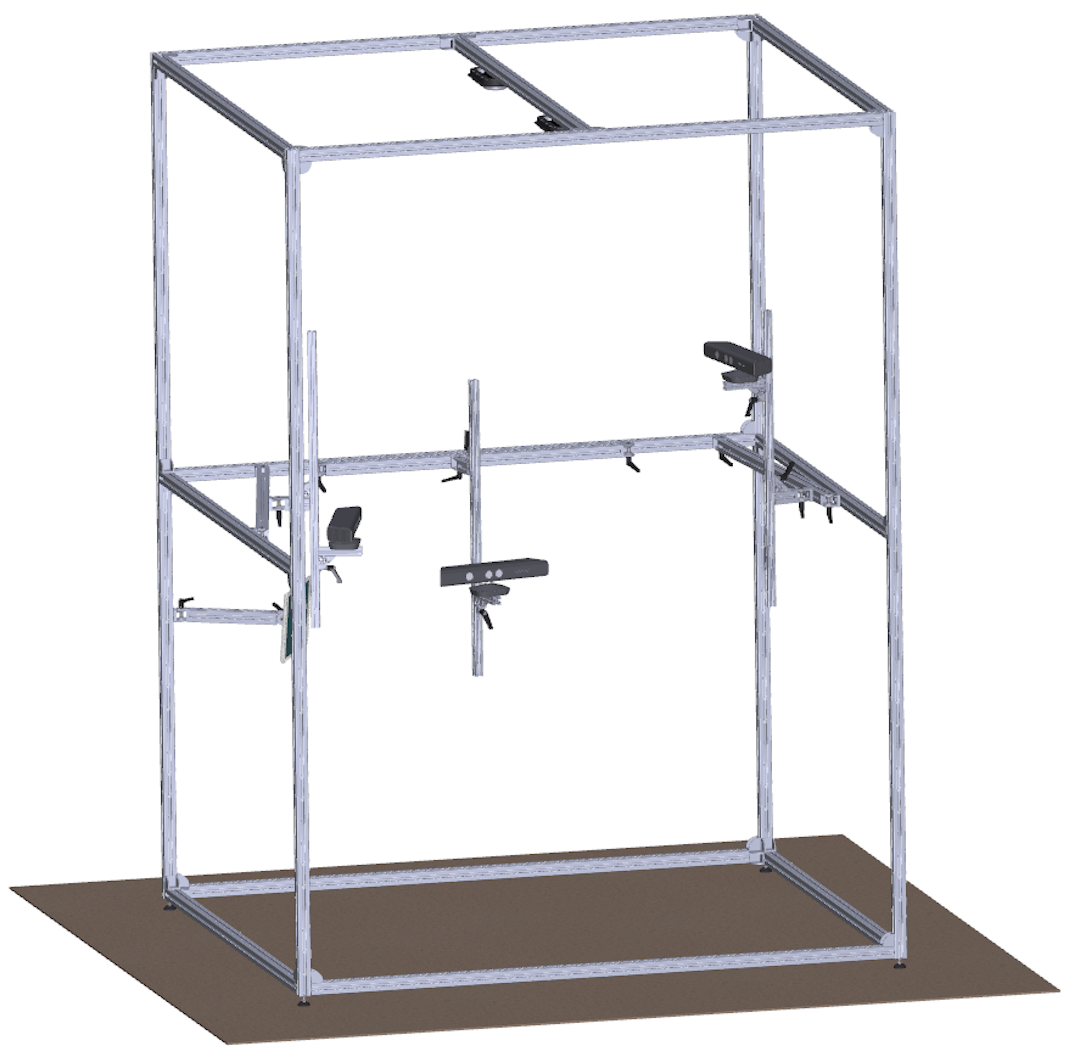
\includegraphics[height=3.5cm]{figures/kinect_cabin.png}
				\caption{}
				\label{fig:cabin}
			\end{subfigure}%
		}\cr
	}
	
	\caption{Referenčné obrazy multi-kamerovej sústavy: (\textbf{a}) RGB snímky. (\textbf{b}) Hĺbkové mapy. (\textbf{c}) 3D model vytvorený z hĺbkových máp. (\textbf{d}) Konštrukcia skenovacej kabíny s ukážkou rozloženia kamier.}
	\label{fig:gt}
\end{figure}

RGB obrázky prijaté z každej kamery sú znázornené na obrázku \ref {fig:gt:a}, hĺbkové snímky snímanej scény bez rušenia (postupne pracujúce kamery) pre jednotlivé kamery sú uvedené na obrázku \ref {fig:gt:b}. Tieto hĺbkové mapy sa použili ako referenčné údaje bez interferenčných artefaktov. Obrázok \ref{fig:reference} je rekonštruovaný 3D model statického objektu.

Aby bolo možné objektívne vyhodnotiť výkon potlačenia rušenia, musí sa identifikovať povaha každého bodu v mračne bodov. Zisťuje či ide alebo nejde o skutočné rušenie. Dáta skreslené interferenciou sa získali v režime paralelného snímania. Pre získanie tejto informácie sme použili priestorové porovnávanie interferovaných dát voči referenčným. Referenčná sieť, znázornená na obrázku \ref {fig:reference}, bola získaná z mračna referenčných bodov. Celkový proces vyhodnotenia metód je uvedený na obrázku \ref{fig:eval}.

\begin{figure}[H]
	\centering
	\includegraphics[width=\textwidth]{figures/eval.png}
	\caption{Blokový diagram vyhodnocovacieho procesu.}
	\label{fig:eval}
\end{figure}

\noindent Kroky v tomto procese sú opísané nasledovne:

\begin{itemize}
	\item \textbf{Zásobník} - zachytenie niekoľkých mračien bodov z konkrétneho pohľadu a zlúčenie do jedného mračna.
	\item \textbf{Filtrovanie} - použitie jednej z metód filtrovania opísaných v podkapitole \ref{sec:filtmethods}.
	\item \textbf{Porovnanie s referenciou} - výpočet Hausdorffových vzdialeností voči referenčnej sieti pre konkrétny pohľad.
	\item \textbf{Priestorové filtrovanie} - štatistické rozhodnutie, či ide o rušenie alebo nie na základe Hausdorffovej vzdialenosti. Za rušenie sa považujú štatistické odľahlé hodnoty.
	\item \textbf{Analýza} - vyhodnotenie výsledkov pomocou známych metrík z ROC analýzy.
\end{itemize}

V experimentálnej časti používame na hodnotenie výkonnosti konkrétnych metód nasledujúce metriky.

\begin{itemize}
	\item \textbf{Accuracy} odráža celkový výkon algoritmu, takže zohľadňuje aj skutočné negatívne predpovede (bod nie je interferovaný). Presnosť je vysoká, keď je počet skutočných pozitívnych a pravdivých negatívnych predpovedí vysoký.
	
	\item \textbf{Recall} predstavuje počet odstránených bodov, ktoré boli interferované. Nezohľadňuje ale počet falošne pozitívnych odstránených bodov. Recall je vysoké, keď je počet skutočných predpovedí (filtrovaných interferenčných bodov) veľký, bez ohľadu na to, koľko užitočných bodov stratíme.
	
	\item \textbf{Precision} odráža počet skutočných predpovedí s ohľadom na počet falošne pozitívnych predpovedí.
	
	\item \textbf{F1 score} je hodnota rovnováhy medzi Recall a Precision. To znamená, že skóre F1 nie je skreslené veľkým počtom skutočne negatívnych predpovedí a môže sa považovať za rozhodujúce.
	
	\item \textbf{Hausdorffova vzdialenosť} meria euklidovskú vzdialenosť dvoch vzájomné porovnávaných bodov. Používa sa stredná hodnota vzdialenosti od bodu v mračne k najbližšiemu povrchu v referenčnej sieti .
\end{itemize}

\section{Výsledky experimentu}

V prvom kroku testovania sa hľadali optimálne nastavenia vstupných parametrov pre jednotlivé filtre. Automatickou rekonfiguráciou sa získali rôzne kombinácie nastavení, z ktorých boli následne vybrané najoptimálnejšie parametre (najlepšie F1 skóre). Vysoká hodnota Accuracy môže byť v tomto prípade zavádzajúci parameter, pretože veľké množstvo TN predikcií skresľuje výsledok. Taktiež nízka Hausdorffová vzdialenosť nemusí automaticky znamenať vysoký výkon filtra. Pri použití Hausforffovej vzdialenosti nevidíme, koľko užitočných bodov bolo zbytočne odstránených. Príklad rozdielu v hodnotení pomocou Hausdorffovej vzdialenosti a F1 skóre je vidieť na obr. \ref{fig:sor_hausdorff}. 


\begin{figure}[h]
	\centering
	\begin{subfigure}[b]{0.32\textwidth}
		\centering
		\includegraphics[height=4cm]{figures/sorinterf.png}
		\caption{}
		\label{fig:sor_hausdorff:a}
	\end{subfigure}
	\hfill
	\begin{subfigure}[b]{0.32\textwidth}
		\centering
		\includegraphics[height=4cm]{figures/soridealfilt.png}
		\caption{}
		\label{fig:sor_hausdorff:b}
	\end{subfigure}
	\hfill
	\begin{subfigure}[b]{0.32\textwidth}
		\centering
		\includegraphics[height=4cm]{figures/soroverfilt.png}
		\caption{}
		\label{fig:sor_hausdorff:c}
	\end{subfigure}
	\caption{Rozdiel v hodnotení výkonnosti filtrácie pomocou Hausdorffovej vzdialenosti a F1 skóre. (\textbf{a}) Mračno bodov s interferenciou. Priemerná Hausdorffova vzdialenosť je veľká. (\textbf{b}) Filtrované mračno bodov. Priemerná Hausdorffova vzdialenosť je nízka a skóre F1 je veľké. (\textbf{c}) Filtrované mračno bodov s veľkou stratou užitočných bodov. Priemerná Hausdorffova vzdialenosť je nízka, skóre F1 je nízke.}
	\label{fig:sor_hausdorff}
\end{figure}

Meranie doby spracovania dát sa uskutočňovalo na operačnom systéme Ubuntu s procesorom Intel® Core ™ i5-6440HQ 2,60 GHz a 16 GB operačnej pamäte. 

\subsection{SOR filtrácia}

Filter SOR nám umožňuje upraviť $sdm$ -parameter (prahová hodnota multiplikátora štandardnej odchýlky) a $k$ -parameter (počet bodov, ktoré sa majú použiť na odhad priemernej vzdialenosti). Nasledujúce farebné mapy (Obr. \ref{fig:sorf1}) ukazujú, ako sa mení výkon filtrácie vyhodnotený ako skóre F1 v závislosti od výberu parametrov a veľkosti vyrovnávacej pamäte.

\begin{figure}[h]
	\centering
	\includegraphics[width=\textwidth]{figures/sor_f1.png}
	\caption{Farebná mapa závislosti F1 skóre od vstupných parametrov SOR filtra pre každú veľkosť obrazového zásobníka.}
	\label{fig:sorf1}
\end{figure}

\begin{table}[h]
	\centering
	\caption{\label{tab:sor_best} Najlepšie výsledky SOR filtrácie pre veľkosti obrazového zásobníka 1-6. }
	\begin{tabular}{cccccc}
		\toprule
		\textbf{Zásobník} & \textbf{Accuracy} & \textbf{Precision} & \textbf{Recall} & \textbf{F1 Score} & \textbf{Priem. HD [m]} \\ 
		\midrule
		\textbf{1}           & 0,964001          & 0,390533           & 0,538043        & 0,452571          & 0,001101           \\ 
		\textbf{2}           & 0,959534          & 0,474334           & 0,719212        & 0,571652          & 0,001073           \\ 
		\textbf{3}           & 0,964936          & 0,472317           & 0,853734        & 0,608171          & 0,001025           \\ 
		\textbf{4}           & 0,951624          & 0,501123           & 0,839413        & 0,627583          & 0,001041           \\ 
		\textbf{5}           & 0,968504          & 0,615551           & 0,754316        & \textbf{0.677905}          & 0,001062           \\ 
		\textbf{6}           & 0,970065          & 0,598705           & 0,76028         & 0,669887          & 0,001053           \\ 
		\bottomrule
	\end{tabular}
\end{table}

Na základe analýzy na obrázku \ref{fig:sorf1} sa získalo najlepšie nastavenie pre filter SOR. Zdá sa, že výkon má stúpajúci trend až do veľkosti zásobníka 5. Ideálna kombinácia parametrov pre veľkosť obrazového zásobníka 5 je $sdm$ 1,5 a $k$ 100. V tomto nastavení algoritmus dosahuje najlepšie skóre F1 0,68, ktoré je vidieť v tabuľke \ref{tab:sor_best}.

\subsection{ROR filtrácia}
\label{sec:ror}
Filter ROR nám umožňuje nastaviť polomer (priestorový rádius použitý na určenie najbližších susedov $pts$) a  $pts$ -parameter (minimálny počet susedov, ktoré musí mať bod v danom polomere vyhľadávania, aby nebol  odfiltrovaný). Nasledujúce farebné mapy znázorňujú, ako sa mení skóre F1 v závislosti od výberu parametrov a veľkosti obrazového zásobníka.

\begin{figure}[H]
	\centering
	\includegraphics[width=0.9\textwidth]{figures/ror_f1.png}
	\caption{Farebná mapa závislosti F1 skóre od vstupných parametrov ROR filtra pre každú veľkosť obrazového zásobníka.}
	\label{fig:rorf1}
\end{figure}

\begin{table}[h]
	\centering
	\caption{\label{tab:ror_best} Najlepšie výsledky ROR filtrácie pre veľkosti obrazového zásobníka 1-6. }
	\begin{tabular}{cccccc}
		\toprule
		\textbf{Zásobník} & \textbf{Accuracy} & \textbf{Precision} & \textbf{Recall} & \textbf{F1 Score} & \textbf{Mean HD [m]} \\ 
		\midrule
		\textbf{1}           & 0,956411          & 0,296154           & 0,418478        & 0,346847          & 0,001116            \\ 
		\textbf{2}           & 0,944072          & 0,352522           & 0,585222        & 0,44              & 0,001104            \\ 
		\textbf{3}           & 0,963341          & 0,446866           & 0,631255        & 0,523293          & 0,001064           \\
		\textbf{4}           & 0,949669          & 0,487503           & 0,711546        & 0,578593          & 0,001092           \\ 
		\textbf{5}           & 0,962245          & 0,553508           & 0,728088        & \textbf{0.628907}          & 0,001068           \\ 
		\textbf{6}           & 0,968228          & 0,590323           & 0,6689          & 0,62716           & 0,001074           \\ 
		\bottomrule
	\end{tabular}
\end{table}

Podobne ako v predchádzajúcom prípade analýza na obrázku \ref{fig:rorf1} ukazuje najlepšie nastavenie pre filter ROR. Výkonnosť filtrácie je najvyššia pre veľkosť zásobníka 5. Ideálna kombinácia parametrov je $rad$ 0,004 a a $pts$ 10. V tomto nastavení dosahuje filter najlepšie skóre F1 0,63, ako je vidieť v tabuľke \ref{tab:ror_best}.

\subsection{PointCleanNet filtrácia}
Pri používaní pred-trénovanej siete PointCleanNet nebolo potrebné zadávať žiadne parametre pre odstraňovanie odľahlých hodnôt. V tomto prípade sa porovnávajú výsledky pre rozdielne veľkosti zásobníka. Spracovanie dát trvalo rádovo v minútach, pričom bola využívaná grafická karta s CUDA podporou.

\begin{table}[h]
	\caption{\label{tab:pcn_best} Najlepšie výsledky PointCleanNet filtrácie pre veľkosti obrazového zásobníka 1-6.}
	\centering
	\begin{tabular}{cccccc}
		\toprule
		\textbf{Zásobník} & \textbf{Accuracy} & \textbf{Precision} & \textbf{Recall} & \textbf{F1 Score} & \textbf{Priem. HD [m]} \\ 
		\midrule
		\textbf{1}           & 0,840448          & 0,084714           & 0,486413        & 0,144297          & 0,00112                         \\ 
		\textbf{2}           & 0,835066          & 0,07334            & 0,291626        & 0,117205          & 0,001226                        \\ 
		\textbf{3}           & 0,830422          & 0,06211            & 0,30639         & 0,103283          & 0,001181                        \\ 
		\textbf{4}           & 0,819131          & 0,096918           & 0,327567        & 0,149579          & 0,001387                        \\ 
		\textbf{5}           & 0,819513          & 0,094805           & 0,363546        & 0,150391          & 0,001324                        \\ 
		\textbf{6}           & 0,823568          & 0,099486           & 0,424307        & \textbf{0,16118}           & 0,001263                        \\ 
		\bottomrule
	\end{tabular}
\end{table}

Výkon filtra má stúpajúci trend so zvyšujúcou veľkosťou zásobníka. Ako je však vidieť z tabuľky \ref{tab:pcn_best}, najlepší výsledok získaný na základe skóre F1 je iba 0,16 pre veľkosť vyrovnávacej pamäte 6.

\subsection{IMBM filtrácia}
\label{sec:imbm:filtration}

IMBM filter umožňuje nastaviť prahovú hodnotu hĺbky (odstránenie pozadia a extréme interferujúcich pixelov), prahovú hodnotu dôležitosti mapy (odstránenie oblastí s nízkou významnosťou pixelov v mediáne hĺbkovej mapy) a šumovú prahovú hodnotu (nastavenie prahovej hodnoty šumu kamery). Optimálna hodnota posledného spomenutého prahu pre veľkosť zásobníka 2 je uvedené na obrázku \ref{fig:imbmth:a} a pre veľkosť zásobníka 6 na obrázku \ref {fig:imbmth:b}. Z analýzy týchto obrázkov je najlepším šumovým prahom pre veľkosť zásobníka 2 hodnota 13 a pre veľkosť zásobníka 6 hodnota 8. Tento parameter bol v ďalšej časti experimentu staticky nastavený na 10.


\begin{figure}[H]
	\centering
	\includegraphics[width=0.85\textwidth]{figures/imbm_th_2.png}
	\caption{Výber ideálneho prahu rozdielu IMBM filtrácie pre veľkosť obrazového zásobníka 2}
	\label{fig:imbmth:a}
\end{figure}

\begin{figure}[H]
	\centering
	\includegraphics[width=0.85\textwidth]{figures/imbm_th_6.png}
	\caption{Výber ideálneho prahu rozdielu IMBM filtrácie pre veľkosť obrazového zásobníka 6.}
	\label{fig:imbmth:b}
\end{figure}

Navrhovaný spôsob filtrovania dosahuje najvyššie F1 skóre pre veľkosť zásobníka 5. V tomto okamihu je zlepšenie priemernej Hausdorffovej vzdialenosti približne o 12 \% (stredná vzdialenosť pre vstupné rušené mračná je 0,001255\,m).

\begin{table}[h]
	\caption{\label{tab:imbm_best} Najlepšie výsledky IMBM filtrácie pre veľkosti obrazového zásobníka 2-6. }
	\centering
	\begin{tabular}{cccccc}
		\toprule
		\textbf{Zásobník} & \textbf{Accuracy} & \textbf{Precision} & \textbf{Recall} & \textbf{F1 Score} & \textbf{Priemerná HD [m]} \\ 
		\midrule
		\textbf{2}           & 0,958461          & 0,433661           & 0,347783        & 0,386003          & 0,001205           \\ 
		\textbf{3}           & 0,978235          & 0,724401           & 0,511932        & 0,59991           & 0,001119           \\ 
		\textbf{4}           & 0,950948          & 0,493889           & 0,410305        & 0,448233          & 0,001229           \\ 
		\textbf{5}           & 0,97733           & 0,815311           & 0,62583         & \textbf{0,708114}          & 0,001114           \\ 
		\textbf{6}           & 0,977306          & 0,807993           & 0,566555        & 0,66607           & 0,001107           \\ 
		\bottomrule
	\end{tabular}
\end{table}

\subsection{Zhodnotenie výsledkov}

Po získaní najlepších nastavení pre konkrétne metódy filtrovania je potrebné komplexne porovnať ich výkonnosti. Obrázok \ref{fig:best} ukazuje vizualizáciu Hausdorffových vzdialeností výstupov z jednotlivých filtrov pre veľkosť zásobníka 5. Toto nastavenie bolo vybrané na základe najlepších výsledkov z tabuľky \ref {tab:final_comp} (s výnimkou PointCleanNet, ktorý dosahuje najlepšie výsledky pri veľkosti 6).

\begin{table}[H]
	\caption{\label{tab:final_comp} Najlepšie skóre F1 pre všetky metódy filtrovania. }
	\centering
	\begin{tabular}{ccccc}
		\toprule
		\textbf{Zásobník} & \textbf{SOR} & \textbf{ROR} & \textbf{PointCleanNet} & \textbf{IMBM}     \\ 
		\midrule
		\textbf{1}           & 0,452571     & 0,346847     & 0,144297               & -                 \\ 
		\textbf{2}           & 0,571652     & 0,44         & 0,117205               & 0,386003          \\ 
		\textbf{3}           & 0,608171     & 0,523293     & 0,103283               & 0,59991           \\ 
		\textbf{4}           & 0,627583     & 0,578593     & 0,149579               & 0,448233          \\ 
		\textbf{5}           & 0,677905     & 0,628907     & 0,150391               & \textbf{0,708114} \\ 
		\textbf{6}           & 0,669887     & 0,62716      & 0,16118                & 0,66607           \\ 
		\bottomrule
	\end{tabular}
\end{table}

\begin{figure}[H]
	\centering
	\begin{subfigure}[b]{0.19\textwidth}
		\centering
		\includegraphics[height=3.5cm]{figures/hausdorff_ref.png}
		\caption{}
		\label{fig:best:a}
	\end{subfigure}
	\hfill
	\begin{subfigure}[b]{0.19\textwidth}
		\centering
		\includegraphics[height=3.5cm]{figures/soridealfilt.png}
		\caption{}
		\label{fig:best:b}
	\end{subfigure}
	\hfill
	\begin{subfigure}[b]{0.19\textwidth}
		\centering
		\includegraphics[height=3.5cm]{figures/ror_best.png}
		\caption{}
		\label{fig:best:c}
	\end{subfigure}
	\hfill
	\begin{subfigure}[b]{0.19\textwidth}
		\centering
		\includegraphics[height=3.5cm]{figures/pcn_best.png}
		\caption{}
		\label{fig:best:d}
	\end{subfigure}
	\hfill
	\begin{subfigure}[b]{0.19\textwidth}
		\centering
		\includegraphics[height=3.5cm]{figures/imbm_best.png}
		\caption{}
		\label{fig:best:e}
	\end{subfigure}
	\caption{Komplexné porovnanie metód filtrácie pomocou vizualizácie vzdialeností medzi filtrovanými mračnami bodov a referenčnou sieťou. (\textbf{a}) Vstupné mračno bodov bez potlačenia rušenia. (\textbf{b}) Najlepší výsledok SOR filtra s parametrami $sdm$ 1.5 a $k$ 100. (\textbf{c}) Najlepší výsledok pri použití ROR filtra s parametrami $rad$ 0.004 and $pts$ 10. (\textbf{d}) Najlepší výsledok pre PointCleanNet filtráciu s veľkosťou obrazového zásobníka 6. (\textbf{e}) Najlepší výsledok pre IMBM filter.}
	\label{fig:best}
\end{figure}

Porovnanie výstupných mračien bodov pre jednotlivé filtračné metódy je zobrazené na obr. \ref{fig:best}. Interferovaná časť objektu obsahovala relatívne komplexné detaily (oči, brada, nos). Filtre pracujúce na princípe štatistiky (SOR, ROR, IMBM) dokázali lepšie odstrániť interferujúce miesta ako filter založený na princípe neurónových sietí (PointCleanNet). Ten odstránil prevažne silno interferované body a mierne potlačil povrchovú interferenciu. Sieť však nebola trénovaná na odstránenie takéhoto typu šumu. Dotrénovaním siete na interferovaných mračnách môže tento filter vykazovať najlepšie výsledky. Je však potrebné vytvoriť dataset interferovaných mračien bodov. SOR a ROR odstránili väčšinu poškodených pixelov. Problém však je, že boli odstránené aj užitočné body, a to práve v miestach interferencie. Takouto stratou nie je možné spätne rekonštruovať poškodené regióny. 

\begin{figure}[h]
	\centering
	\begin{subfigure}[b]{0.3\textwidth}
		\centering
		\includegraphics[width=0.6\textwidth]{figures/ball_mesh.png}
		\caption{}
		\label{fig:ball:a}
	\end{subfigure}
	\hfill
	\begin{subfigure}[b]{0.3\textwidth}
		\centering
		\includegraphics[width=\textwidth]{figures/ball_interf.png}
		\caption{}
		\label{fig:ball:b}
	\end{subfigure}
	\hfill
	\begin{subfigure}[b]{0.3\textwidth}
		\centering
		\includegraphics[width=\textwidth]{figures/ball_imbm.png}
		\caption{}
		\label{fig:ball:c}
	\end{subfigure}
	\hfill
	\newline
	\vfill
	\begin{subfigure}[b]{0.3\textwidth}
		\centering
		\includegraphics[width=\textwidth]{figures/ball_sor.png}
		\caption{}
		\label{fig:ball:d}
	\end{subfigure}
	\hfill
	\begin{subfigure}[b]{0.3\textwidth}
		\centering
		\includegraphics[width=\textwidth]{figures/ball_ror.png}
		\caption{}
		\label{fig:ball:e}
	\end{subfigure}
	\hfill
	\begin{subfigure}[b]{0.3\textwidth}
		\centering
		\includegraphics[width=\textwidth]{figures/ball_imbm_sor.png}
		\caption{}
		\label{fig:ball:f}
	\end{subfigure}
   \caption{Vizualizácia Hausdorffovej vzdialenosti pre IMBM, SOR a ROR filtre. Všetky výsledky sú pre veľkosť obrazového zásobníka 5. (\textbf{a}) Referencia (lopta). (\textbf{b}) Rozdiel medzi interferenciou a lietajúcimi bodmi. (\textbf{c}) Potlačenie interferencie IMBM filtrom, lietajúce doby ostali.  (\textbf{d}) SOR filter odstránil lietajúce body ale interferencia ostala.  (\textbf{e}) ROR filter odstránil lietajúce body ale interferencia ostala. (\textbf{f}) Najlepší výsledok aplikovaním IMBM a SOR filtra spoločne.}
\label{fig:ball}
\end{figure}

Problematickými časťami filtrov SOR a ROR sú rohy a hrany, ktoré sa filtrovaním zaobľujú. Ako je uvedené v štúdii \cite{Pirotti}, filter SOR vníma body na hranách ako odľahlé body. Tieto filtre tiež odstraňujú malé ostrovy bodov (zhluky bodov, ktoré nie sú bodmi rušenia) \cite{Schaller}. Ako je uvedené v \cite{Balta}, filtrovanie SOR nie je úplne vhodné pre výkon v reálnom čase. IMBM filter dokázal potlačiť interferenciu bez väčšej straty plochy objektu, čo je znázornené aj na obr. \ref{fig:best:e}. IMBM sa nezameriava iba na odstraňovanie rušenia, ale poskytuje aj interpoláciu chýbajúcich bodov, avšak výrazne predlžuje dobu spracovania dát. Nedokázal ani odstrániť všetky chybné body. Je to spôsobené tým, že tieto body boli podobné vo všetkých hĺbkových mapách v obrazovom zásobníku. Pre elimináciu chybných dát a zníženie Hausdorffovej vzdialenosti je možné kombinovať IMBM filter s inými štatistickými filtrami.

Na záverečné vyhodnotenie metód filtrovania sa použil dataset zložený z 23 objektov. Tento nami vytvorený dataset obsahuje 23 skenov predmetov (guľa, plastová fľaša ...) zachytených z rôznych pohľadov. Nasledujúca tabuľka \ref{tab:dataset} zobrazuje mediány každej vyhodnocovanej metriky v celom datasete. Všetky výsledky sú pre veľkosť obrazového zásobníka 5.

Na základe výsledkov tohto prieskumu je odporúčané používať metódy filtrovania pre konkrétne aplikácie podľa ich funkcií opísaných v tabuľke \ref{tab:functionality}.


\begin{table}[h]
	\caption{\label{tab:dataset} Medián všetkých použitých metrík v celom datasete. }
	\centering
	\begin{tabular}{cccccc}
		\toprule
		\textbf{Metóda}     & \textbf{Accuracy} & \textbf{Precision} & \textbf{Recall}   & \textbf{F1 score}          & \textbf{Priemerná HD [m]} \\
		\midrule
		SOR        & 0.936164 & 0.980778  & 0.393617 & 0.555951          & 0.002393               \\
		ROR        & 0.927161 & 0.639983  & 0.734787 & 0.647839          & 0.001697               \\
		PCN        & 0.862285 & 0.371242  & 0.472615 & 0.409729          & 0.00221                \\
		IMBM       & 0.908833 & 0.673608  & 0.442942 & 0.477348          & 0.002563               \\
		IMBM + ROR & 0.918448 & 0.59806   & 0.820666 & 0.653113          & 0.001656               \\
		IMBM + SOR & 0.943387 & 0.704448  & 0.836253 & \textbf{0.741811} & 0.001548   \\    \bottomrule  
	\end{tabular}
\end{table}

\begin{table}[h]
	\caption{\label{tab:functionality} Porovnanie vlastností filtračných metód }
	\centering
	\begin{tabular}{cccccc}
		\toprule
		\textbf{Metóda} & \textbf{Potláč. interf.} & \textbf{Rýchlosť} & \textbf{Filtrovanie hrán/rohov} & \textbf{Obnova dát} \\ 
		\midrule
		\textbf{SOR}     & Stredná      & Stredná    & Stredná   & Nie    \\ 
		\textbf{ROR}     & Stredná      & Vysoká      & Stredná   & Nie    \\ 
		\textbf{PCN}     & Nízka       & Nízka       & Stredná   & Ano   	\\ 
		\textbf{IMBM}    & Vysoká      & Vysoká      & Nízka      & Ano   \\ 
		\bottomrule
	\end{tabular}
\end{table}

Ideálnou voľbou je použitie IMBM filtra pre potlačenie interferencie spolu s ROR alebo SOR filtrom pre odstránenie zvyšných chybných bodov. IMBM a SOR filtre boli aplikované v kapitole \ref{sec:filtration}. 